\documentclass[a4paper]{article}
\usepackage[utf8]{vietnam}
\usepackage[left=80pt,right=80pt,top=60pt,bottom=60pt]{geometry}
\usepackage[font=small,labelfont=bf]{caption}
\usepackage{graphicx}
\usepackage{amssymb}
\usepackage{amsmath}
\usepackage{array}
\usepackage{hyperref}

\graphicspath{ {./imgs/} }

\newcolumntype{L}{>{\centering\arraybackslash}m{2cm}}
\newcolumntype{M}{>{\centering\arraybackslash}m{6cm}}

\hypersetup{
    colorlinks=true,
    linkcolor=magenta,     
    urlcolor=cyan,
}

% \setlength{\parskip}{1em}

\title {
    BÀI BÁO CÁO NHÓM 10\\
    MÔ PHỎNG THÍ NGHIỆM PHÂN ĐOẠN TỪ TRONG TÀI LIỆU VIẾT TAY BẰNG KỸ THUẬT SCALE SPACE
}

\author {
    Nguyên tác: \textit{R. Manmatha và Nitin Srimal}\\
    Bài báo gốc: \url{http://ciir.cs.umass.edu/pubfiles/mm-27.pdf}\\
    Thành viên nhóm 10:
    \begin{tabular}{ l l }
        Nguyễn Vũ Bình Dương & 19020060 \\
        Vũ Ngọc Hiển & 19021268 \\ 
        Ngô Văn Huy & 19001304
    \end{tabular}
}


\begin{document}

\maketitle
\pagebreak

\tableofcontents
\pagebreak

\section*{Tóm tắt}
\addcontentsline{toc}{section}{Tóm tắt}
Thí nghiệm này phỏng theo thí nghiệm, bài báo khoa học của R. Manmatha và Nitin Srimal [1]. Mục đích của thí nghiệm này là hỗ trợ số hóa các tài liệu viết tay của con người, cụ thể là trích xuất được các hình ảnh con chứa từng từ trong văn bản cho trước. Thuật toán để làm được điều này được thực hiện bằng cách chia một ảnh văn bản nhiều dòng thành các ảnh con, mỗi ảnh con chứa một dòng duy nhất từ văn bản gốc, sau đó làm đậm các chữ cái liên thông với nhau để trích xuất được vị trí chính xác của từng từ trong dòng đó.

\section{Dữ liệu}
\label{sec:1}
Bộ dữ liệu được dùng để thí nghiệm và phân tích được lấy trên google, là những bức ảnh chứa văn bản viết tay bằng tiếng Anh, viết theo cấu trúc văn bản, cách dòng thông thường (\ref{fig:fig1}). Đa phần các bức ảnh trong bộ dữ liệu đều không có kẻ dòng sẵn, đồng thời cũng đã được tiền xử lý để loại bỏ các chi tiết thừa như logo, con dấu, \ldots sau đó được đọc trên kênh màu xám để thuận tiện cho thí nghiệm tập trung vào thuật toán tách dòng và từ trong văn bản.

\begin{figure}
    \centering
    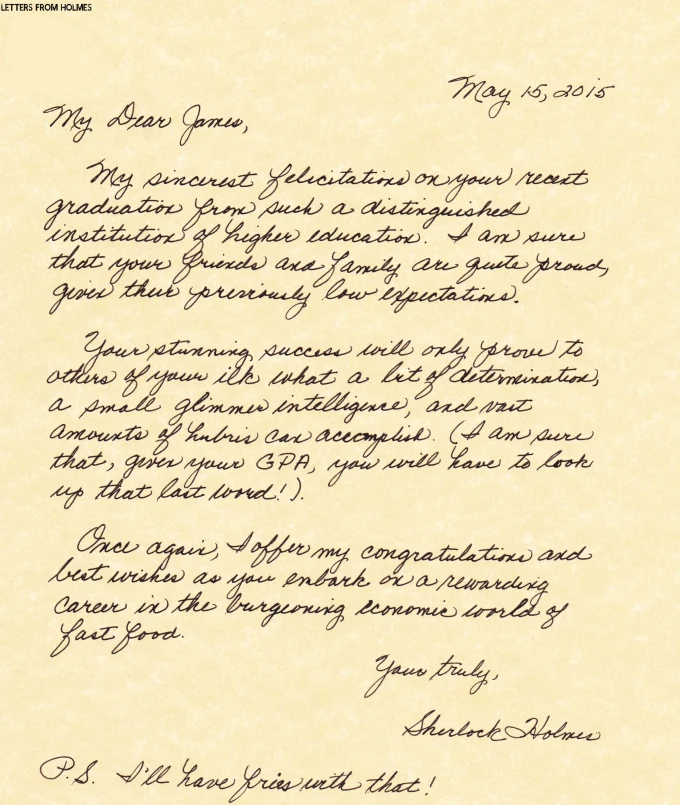
\includegraphics[width=0.5\textwidth]{letter_from_holmes.png}
    \caption{Ảnh một bức thư tay}
    \label{fig:fig1}
\end{figure}

\pagebreak

\section{Tách dòng}
\label{sec:2}

\begin{figure}
    \centering
    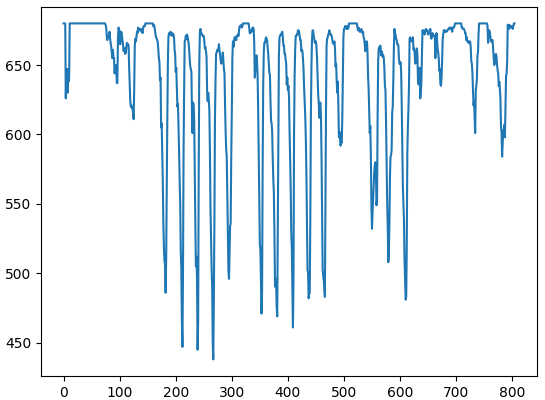
\includegraphics[width=0.5\textwidth]{projection1d.png}
    \caption{Ảnh plot tín hiệu 1 chiều của ảnh 2D}
    \label{fig:fig2}
\end{figure}

\begin{figure}
    \centering
    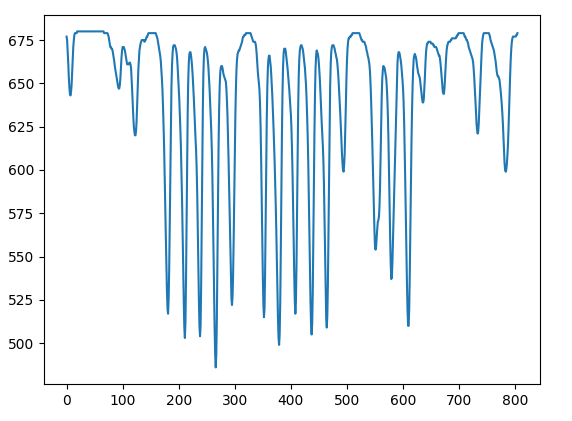
\includegraphics[width=0.5\textwidth]{gauss1d.png}
    \caption{Ảnh plot tín hiệu 1 chiều của ảnh 2D sau khi qua bộ lọc Gaussian}
    \label{fig:fig3}
\end{figure}

Đầu tiên ảnh sẽ được chuyển qua dạng nhị phân với threshold cơ bản là 127, sau đó được chiếu vào một mảng để chuyển thành tín hiệu 1 chiều như sau: khởi tạo một mảng $G$ có kích thước bằng chiều cao của ảnh, mỗi phần tử có giá trị bằng chiều rộng của ảnh, sau đó xét từng điểm ảnh, nếu điểm ảnh tại vị trí $(x, y)$ có giá trị bằng 0 (màu đen tức là có vết mực ở đó) thì ta cập nhật giá trị cho mảng $G$ tại vị trí thứ $y$. Sau khi chuyển sang được tín hiệu 1 chiều, tín hiệu được plot ra sẽ trông như hình~\ref{fig:fig2}\par

Ta có thể thấy trên bức ảnh, dòng nào càng nhiều chữ (nhiều vết mực) thì trên đồ thị ~\ref{fig:fig2} tín hiệu sẽ mạnh hơn (nhô lên cao hơn) tương ứng với vị trí của dòng đó. Tuy nhiên, biểu đồ này còn quá nhiều điểm cực trị nên cần làm mịn tín hiệu bằng phép lọc Gaussian như ta đã được học. Sau khi làm mịn tín hiệu biểu diễn ra được như hình~\ref{fig:fig3}, số lượng điểm cực trị đã được giảm xuống, chỉ còn các điểm cực trị tương ứng với vị trí của dòng chữ trên văn bản. Ta chiếu lại vị trí của các cực trị này lên ảnh nhị phân cho ra kết quả rất chính xác như hình~\ref{fig:fig4}:

\begin{figure}
    \centering
    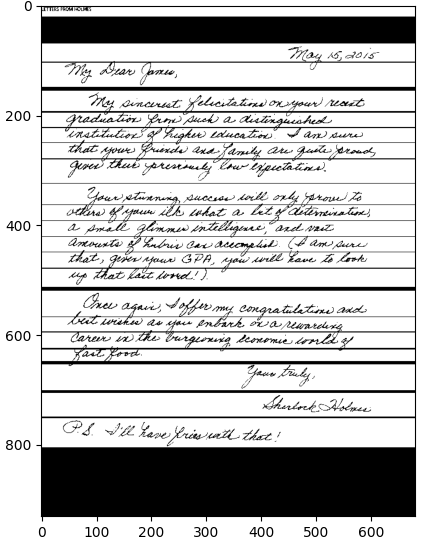
\includegraphics[width=0.5\textwidth]{mapline.png}
    \caption{Chiếu các cực trị thu được vào ảnh nhị phân để chia dòng}
    \label{fig:fig4}
\end{figure}

\pagebreak

\section{Tách từ}
\label{sec:3}

Sau khi có được ảnh nhị phân của từng dòng chữ, ta tiến hành tách từ bằng cách làm đậm các chữ cái trong từ đó lên để tạo ra các blob, mỗi blob như một đốm mực tạo từ các pixel màu đen. Để làm đậm các từ, ta dùng bộ lọc Gaussian dị hướng, công thức của bộ lọc này như sau:

\begin{equation*}
    G(x, y; \sigma_x, \sigma_y) = \frac 1{2\pi \sigma_x\sigma_y} e^{-(\frac {x^2}{2\sigma_x^2} + \frac {y^2}{2\sigma_y^2})}
\end{equation*}
    $(x, y)$: Tọa độ của điểm x, y trong bộ lọc\\
    $\sigma_x, \sigma_y:$ tỷ lệ độ lệch, quyết định độ đậm nhạt của blob

Khi áp dụng, ta dùng bộ lọc là hàm vi phân bậc 2 của công thức phía trên như trong bài báo mà tác giả đã đề cập:

\begin{equation*}
    L(x, y; \sigma_x,\sigma_y) = G_{xx}(x, y; \sigma_x, \sigma_y) + G_{yy}(x, y; \sigma_x, \sigma_y)
\end{equation*}

\begin{figure}[b]
    \centering
    
\includegraphics[width=0.5\textwidth]{line9.png}
    \caption{Dòng 9 của lá thư sau khi nhân chập cho ra các blob, $\sigma_x = 16, \sigma_y = 4$}
    \label{fig:fig5}
\end{figure}

Bộ lọc này sau đó được nhân chập với ảnh nhị phân của một dòng chữ, khi thực hiện, ta chọn $\sigma_x = 16, \sigma_y = 4$ vì theo tác giả đây là tỷ lệ cho ra kết quả tốt nhất. Hình~\ref{fig:fig5} là dòng số 9 trong lá thư sau khi được nhân chập với bộ lọc Gaussian dị hướng, ta có thể thấy các blob đã được tách bạch tương ứng với từng từ trong dòng chữ này.\par

\begin{figure}
    \centering
    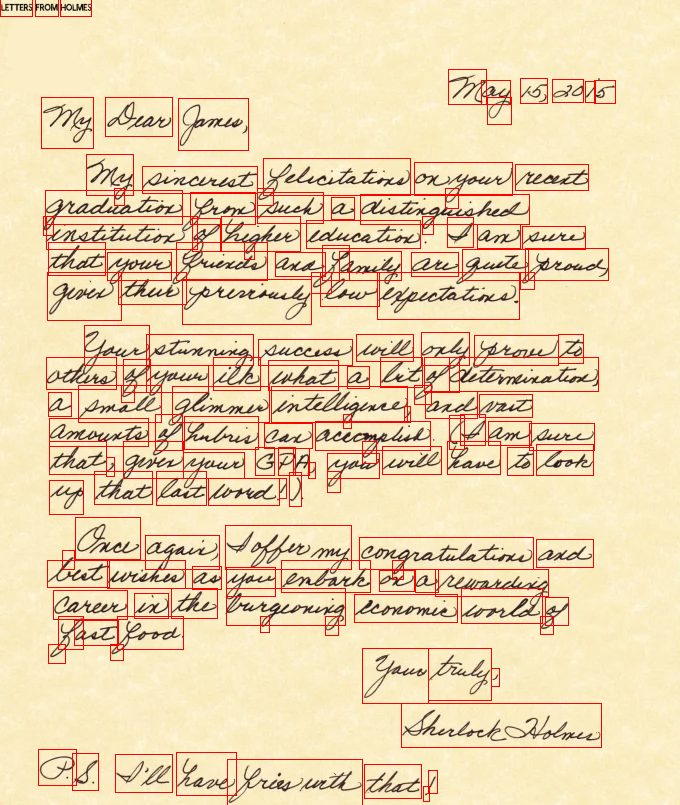
\includegraphics[width=0.5\textwidth]{boxes.png}
    \caption{Kết quả phân đoạn từ bằng kỹ thuật scale space}
    \label{fig:fig6}
\end{figure}


Ta trích xuất vị trí của các blob này bằng thuật toán loang ma trận, một lần loang ta ghé thăm hết các ô màu đen (ô có mực) trên ảnh nhị phân, như vậy ta tìm được tung độ nhỏ nhất, tung độ lớn nhất, hoành độ nhỏ nhất, hoành độ lớn nhất của blob đó. Map lại tọa độ của các blob vào ảnh gốc, ta được kết quả như hình~\ref{fig:fig6}

\pagebreak
\section{Kết luận}
Sau đây là kết quả đạt được khi thực nghiệm với 10 ảnh viết tay(đây là kết quả sau khi kiểm tra và đếm bằng tay):
\begin{center}
    \begin{tabular}{|c|c|c|c|} 
        \hline
        STT & Số từ trong ảnh & Số từ phát hiện đúng & Số phát hiện lỗi \\ 
        \hline
        1 & 120 & 112 & 19 \\
        \hline
        2 & 117 & 113 & 27 \\
        \hline
        3 & 35 & 36 & 5 \\ 
        \hline
        4 & 170 & 160 & 100 \\ 
        \hline
        5 & 117 & 121 & 28 \\ 
        \hline
        6 & 61 & 55 & 9 \\ 
        \hline
        7 & 34 & 30 & 13 \\ 
        \hline
        8 & 36 & 34 & 12 \\ 
        \hline
        9 & 9 & 9 & 0 \\ 
        \hline
        10 & 112 & 77 & 31 \\ 
        \hline
        Tổng & 811 & 747 & 244 \\ 
        \hline
    \end{tabular}
\end{center}
Độ chính xác đạt được là xấp xỉ 92.1\%, cao hơn một chút so với trong bài báo(87.6\%), lí do là vì sample được lấy khá lí tưởng và số lượng sample nhỏ.
Tuy nhiên, đây chỉ là các trường hợp mà các chữ được viết theo dạng nối với nhau. Đối với trường hợp chữ viết cách xa nhau và không có nét nối thì gần như ta không phát hiện được đúng từ nào, ví dụ như ở hình \ref{fig:fig7}.
Ta có thể kết luận được rằng phương pháp này có một điểm hạn chế là không áp dụng được cho những chữ viết tay "cụt", không có nét nối giữ các chữ trong một từ.
\begin{figure}
    \centering
    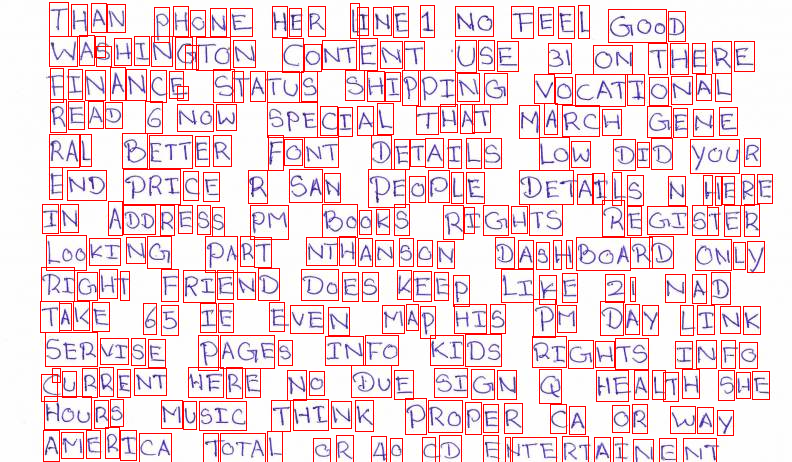
\includegraphics[width=0.5\textwidth]{failure.png}
    \caption{Trường hợp đặc biệt}
    \label{fig:fig7}
\end{figure}


\label{sec:4}

\end{document}
